%-----------------------------------------------------------
%Presentation
\chapter{Presentation}
\section{Stanford University, Palo Alto}

\begin{figure}[!h]
\begin{center}
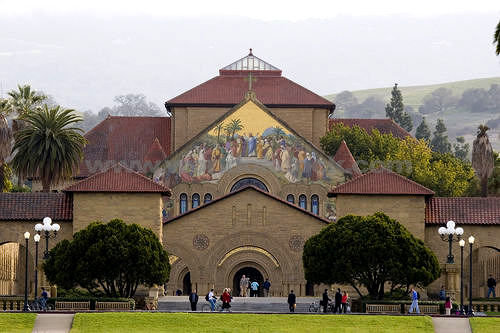
\includegraphics[scale=0.65]{images/stanford.png}
\caption{\small Stanford University, Palo Alto}
\end{center}
\end{figure}
\par
Leland Stanford Junior University (commonly referred to as Stanford University) is a private research university located in the San Francisco Peninsula, more exactly in Palo Alto, California, United States. Stanford was founded in 1885 by former California governor and Senator Leland Stanford as a memorial to his son Leland Stanford Jr. The Stanfords used their farm lands to establish the university hoping to create a large institution in California. The campus is the largest campus in the world, in terms of contiguous acreage with 33.1 km\textsuperscript{2}.
\par
Today, Stanford enrolls about 6,500 undergraduate and about 10,000 graduate students from the United States and around the world every year.
\par
The university is divided into seven schools: School of Humanities and Sciences, School of Engineering, School of Earth Sciences, School of Education, Graduate School of Business, Stanford Law School and the Stanford University School of Medicine.
\par 
In the world, Stanford is one of the most highly regarded schools. Thus, in 2008, it was ranked 2th in the world by the annual list, Top 500 World Universities, published by the Institute of Higher Education at Shanghai Jiao Tong University, China.
\par
The University has a significant impact in the world of research with a lot of research centers and with one of the most important research spending in the world. Moreover, current community of scholars includes a large number of high awarded researchers among them, 18 Nobel Prize and 135 members of the National Academy of Sciences. As part of the Silicon Valley, its alumni have founded companies like Hewlett-Packard, Sun Microsystems, Nvdia, Yahoo!, Cisco Systems and Google.

\section{Department of Psychology}
\par
The department is organized into five different areas of study within the field of psychology. They are: Cognitive, Developmental, Neuroscience, Personality and Social Psychology. 
\par
Currently there are many different kinds of research studies being conducted in this department, on such topics as aggression, social behavior, competitiveness, dreaming, color perception, spatial relations, learning and memory. Researchers rely on participants to keep this research going.
\par
Neuroscience investigates the human brain, from the functional organization of large scale cerebral systems to microscopic neurochemical processes. Topics include the neural substrates of perception, attention, memory, language, learning, neurological disorders, affect, stress and motivation. A variety of experimental techniques are used, including functional magnetic resonance imaging (fMRI), electro/magneto-encephalogry (EEG/MEG), and transcranial magnetic stimulation (TMS). 

\section{VISTA laboratory}
Stanford’s Vision, Imaging Sciences and Technology Activities (VISTA) laboratory is a major research center focused on the use of neuroimaging methods (fMRI, DTI) and behavior to study the human visual system. It is part of the department of Psychology of  Stanford university.
\par
The center’s current research portfolio encompasses projects across several technologies and applications areas, examples of which include:
\begin{itemize}
\item Color vision: the team uses both neuroimaging and behavior testing to understand the action of the visual portions of the brain. They have developed a set of methods for identifying and measuring distinct and specialized regions of human visual cortex, including regions that respond powerful to motion and color.
Image systems: this work is to support multidisciplinary training, research and collaboration on technologies leading to novel imaging systems that include the capture, processing, transmission and rendering of visual information.
\item Reading development: the laboratory is applying a powerful set of measurement methodologies to study human brain development. In one group of studies, they are measuring the signals and growth of visual cortex in children, aged 8-12, during the period children become skilled readers. Using very high spatial resolution and neuroimaging techniques, including some methods developed by this group, they are hoping to understand how visual signals contribute to the neural pathways of reading.
\end{itemize}
\par
For their researches, they have developed several tools regrouped in an overall software tool called mrVista (Mister Vista). This software includes methods for processing anatomical, functional and diffusion tensor imaging data. It is written mainly in Matlab. Other softwares have been developed by the team. Among them, ITKGray is a tool for segmentation and CINCH is a tool for visualization and segmentation of tractography results into meaningful fiber bundles.
\par
More information about the researches conducted by the team and their softwares is given on the website: http://white.stanford.edu. 

\section{Presentation of the overall project}
\subsection{Problematic}
\par
As explain before, the main goal of the project is to answer to the problems of data management met by a lot of research centers around the world, especially in the field of neurosciences, where the amount of data is huge. These problems are similar in other fields of research such as genomics with for example, the Human Genome Project database and the Protein Data Bank or in astronomy where a lot of work are made around the management of data. For example, the Sloan Digital Sky Survey is making an increasing use of DBMS technology to describe millions of celestial objects, and to enable searches across that data (Nieto-Santisteban et al, 2005).
\par
In the field of neuroscience, these problems have already been studied by several groups of researchers and some of them have produced interesting works as the CNARI project: The Computational Neuroscience Applications Research Infrastructure, fMRIDC: The Functional Magnetic Resonance Imaging Data Center or XNAT: The Extensible Neuroimaging Archive Toolkit. Details about these projects and some others will be given further in this document as an inventory on the domain.
\subsection{Objectives and hindrances}
\par
Nevertheless, the need and the possibility to improve considerably the storage, sharing, mining and analysis of the neuroimaging data still exists and significant improvements will come with the multiplication of system of data management. In this purpose, we would like to create a new data system management called: NIMS: Neurobiological Image Management System, which will be used and shared in a first step by all the laboratories of Stanford University working on the neuroscience, most of them part of the Psychology Department. As last step, the system might be extended to other laboratories. Indeed, we use an open-source approach thanks to a common language (Python) to allow an easy deployment and an easy arrangement in contradiction with  current project as CNARI, which use their own language (Swift).
\par
Thus, with this work, the Vista laboratory would like to improve considerably the researcher and team productivity by supporting a new neurobiological imaging workflow and by allowing an expansion in the types and the complexity of questions we are able to ask to the system. Another goal is to allow a collaborative research through several research centers. Indeed, the members of the laboratory believe that sharing information (images, results of analysis) between laboratories will permit to facilitate and increase the number of new findings in  neuroscience. The figure 1.2 shows an overall view of NIMS. As explain, data from scanners, processed images and related measures should be able to be loaded in NIMS. Local user and collaborators should be able to retrieve these data.
\begin{figure}[!h]
\begin{center}
\includegraphics[scale=0.7]{images/nims_overview.png}
\caption{\small NIMS: overall view}
\end{center}
\end{figure}
\par
However, with this project, we face several problems. First of all, the backup of images and research results are necessary for system like ours. Then, a work asking for a collaboration between research centers is often difficult to set in place because of the differences of point of view and of course the differences in the process, especially here in the image workflow (data format and conversion, image nomenclature, etc). Another thing is the problems of security and access control which are essential to protect the patients involved in the research and to respect the privacy and the work of each laboratory.
\subsection{Initial road map}
\par
The initial road map consists in three main parts. First, we have to establish the requirements from major stakeholders by understanding the neuroimaging workflow in each laboratory (image format used, steps followed to store images, etc), by understanding pain points in each workflow and by capturing productivity improvement opportunities to create a new optimized workflow. The second part consists on the definition and the design of the NIMS architecture. The initial functionality of the system are an iterative refinement of raw scanner data into standardized images representations and the implementation of basic workflow analysis. At this step, we will have to create a new ontology of lab images and research results to allow to put user-defined attributes on images and thus, answer to the needs of each laboratory and increase the complexity of questions we will be able to ask. Then, the team will think for additional feature sets to add to the system such as the possibility to index images and research results by region. Finally, the NIMS system will be implemented in real condition for testing purposes. Of course, after this work, the team will be attached to allow the system to be shared with external research centers working on neuroscience especially in the field of fMRI.






